%!TEX root = ../Thesis.tex
\chapter{Crosstalk Experiments}
\label{chap:experiments}
In this section we discuss the details of thorough experiments that we conducted in order to quantify how the crosstalk affects the perceived depth. For the sake of completeness, we performed various experiments on considerably complex (realistic looking) rendered images that consisted of stimuli of various widths and geometric complexities. The effects of crosstalk were observed for both stereoscopic and automultiscopic displays.

\section{Motivation}
 Some preliminary work has been done by Tsirlin et al \cite{tsirlin2011effect}\cite{tsirlin2012crosstalk}\cite{tsirlin2012effect} in order to understand these effects. However, several aspects of their experiments were somehow limited for the aim of applying the findings in a practical scenario. Firstly their experiments were performed on monochromatic images where no depth cues other than disparity were present. As mentioned in Chapter 3, we conducted a pilot experiment using such stimuli (a thin rectangular white bar on a black background) using a similar Wheatstone setup (Figure \ref{fig:wheatstone_setup}) and found that it was very hard to sense any depth of the stimulus even at high disparities. Even after some time, guessing the apparent distance of the stimulus from the screen in length units was quite unreliable. This would be an indicative that the naive test subjects in their experiments may also have encountered the same problems. This observation is backed by the fact that the test subjects in \cite{tsirlin2012effect} and \cite{tsirlin2011effect} reported reduced depth of the stimuli even when no crosstalk was present. More reliable experiments would be ones where the test subjects report the actual theoretical depth in the base case, i.e., when no crosstalk is present. Additionally, the test subjects were simply asked to report the perceived depth via a sliding bar representing zero or some maximum depth at extremes of the bar; this methodology, relying on the subjects choosing within a scale is susceptible to varying answers both intra-subject, and especially, inter-subjects. Further, the scenes of the natural world usually have at least some other monocular cues e.g. proper light shading, texture gradients, defocus blur etc. Finally, since one factor contributing to visibility of the ghosts is also how much it is separated from the object, wide objects at some disparity will exhibit less visible ghosting than thin stimuli. For these reasons, we decided to use a more reliable, reference matching experimental setup to analyze the effects of crosstalk on the observed depth on rendered stimuli of different widths in a natural scene.

It is commonly believed that the reason for degraded observed depth in the presence of crosstalk is due to the fact that the human visual system is confused in choosing the exact location (or disparity) of the correct match for an object in the corresponding binocular retinal image. To the best of our knowledge, it was unclear whether this HVS confusion is elevated or reduced when the geometric complexity of the object (stimulus) is increased. For this reason, we set out to analyze the crosstalk effects on depth perception of geometrically complex stimuli. Another motivation for our proposed thorough analysis of crosstalk effects on perceived depth of thin stimuli was, that, current studies suggest that for a certain crosstalk level and considerably smaller width of a disparate object, the extent of observed depth degradation increases as the disparity increases. This sounds counter-intuitive because, for substantially high disparity of a thin object, the ghost will be completely separated and located far away from the actual object itself. If, the reason for degraded depth is actually the confusion of HVS in finding the proper match (for an object in one retinal image) between the actual stimulus and its ghost in the corresponding retinal image, then in this case (thin stimulus and large enough disparity), the HVS should be able to find the proper match relatively easily. The reason being that, intuitively, it should be easier to distinguish between the ghost and the stimulus when they are completely separated as compared to the case of overlapping ghost. We hypothesized that the observed depth (when viewed on a stereoscopic display containing some level of crosstalk) of any object with respect to the actual theoretical depth should degrade as long as some part of its ghost overlaps the object itself. However, the observed depth should improve when the ghost separates completely. Hence the graphs of Figure \ref{fig:tsirlin_res} should be parabolic shaped.

In stereoscopic displays, the arrangement of object-ghost pair is antisymmetric between the eyes. This, however, is not the case with automultiscopic displays. As seen in Figure \ref{fig:gaussians}, at least two of the neighboring views are responsible for adding crosstalk at any viewing position. Also, at the sweet spots, the number of views involved in light leakage from the left is always equal to the number of light leaking views from the right. Because the automultiscopic display shows light fields, the arrangement of object-ghost tuple is symmetric in both eyes (at sweet spots). This is a major difference when compared to stereoscopic displays and it is possible that the HVS reacts differently to depth perception in an automultiscopic display. To the best of our knowledge, until now, there have been no studies that observed the effect of crosstalk on perceived depth in automultiscopic displays. For this reason we decided to analyze the effects of an automultiscopic display's sweet spot crosstalk on the perceived depth of all the stimuli we used in experiments for the stereoscopic case.

\section{Stimuli}
Our stimuli consisted of an object (a cylinder or a dragon) placed in front of a plane that had a wooden texture. The reason for choosing a textured background was the HVS's efficiency in distinguishing between textures. This would make it easier for the observer to correctly guess the distance between the background and the foreground object. In order to make sure that our stimuli contained most of the basic monocular cues, we rendered them using a rendering system (Blender  version 2.73).
The scene (coordinates represented in meters) as shown in Figure \ref{fig:blender_scene}, consisted of an object of interest placed at origin. The background plane with wooden texture was placed 3 meters behind the object parallel to the camera plane. In order to capture the shading effects on the object, the scene was lit with a light source (sun) that was placed 10 meters in front and 3 meters at height of the object. Finally the camera was 10 meters in front of the object.The stereo scene was generated by capturing the two images at some distance on each side parallel to the image plane. This distance represented the baseline of the cameras, and was varied.

Our experiments were based on test subjects judging the observed distance between the cylinder and the textured plane. This could have been achieved by either moving the cylinder or by moving the background plane in space relative to the camera. However, this would have changed the object or the texture size which could have been used as an undesired (not affected by crosstalk) cue by the observers. In order to avoid that, we simply generated a dense series of images with varying camera baselines and keeping the position of the background plane in lock with respect to the camera. This way, the background was always at zero disparity (i.e. the plane of focus) and the cylinder always had a crossed disparity (proportional to the baseline distance) meaning the cylinder always appeared to be in front of the plane at different distances. In order to avoid resizing while being displayed on our display, images were rendered at the resolution of 768$\times$432 pixels. With the smallest baseline, the observed distance between the cylinder and the plane was negligible whereas this distance appeared to be increasing as the baseline increased, while keeping the size of object, size of texture and the proximity of the object to the texture constant. For the objects we chose four cylinders of different radii and a dragon from Stanford's 3D scanning repository\footnote{http://graphics.stanford.edu/data/3Dscanrep/}. Figure \ref{fig:stimuli_stereo} shows a sample. The details of each of the objects can be found in Table \ref{tab:stimili_desc}.
\begin{table}[ht!]
  \begin{center}
    \caption{Description of the objects used as stimuli.}
    \label{tab:stimili_desc}
    \begin{tabular}{ccc}
      \toprule
      Object & Scene Dimensions (xyz) & On-screen Dimensions (arc min)\\
      \midrule
      Cylinder(thin) & 5cm x 2m x 5cm & 18.9 x 357\\
      Cylinder(medium) & 10cm x 2m x 10cm & 37.8 x 357\\
      Cylinder(thin) & 45cm x 2m x 45cm & 56.7 x 357\\
      Cylinder(thickest) & 80cm x 2m x 80cm & 75.6 x 357 \\
      Dragon & 0.31m x 0.22m x 14.17cm & 380 x 260.4 (max) \\
      \bottomrule
    \end{tabular}
  \end{center}
\end{table}

\begin{figure}[htbp]
% \centering
    \begin{subfigure}[b]{0.5\textwidth}
        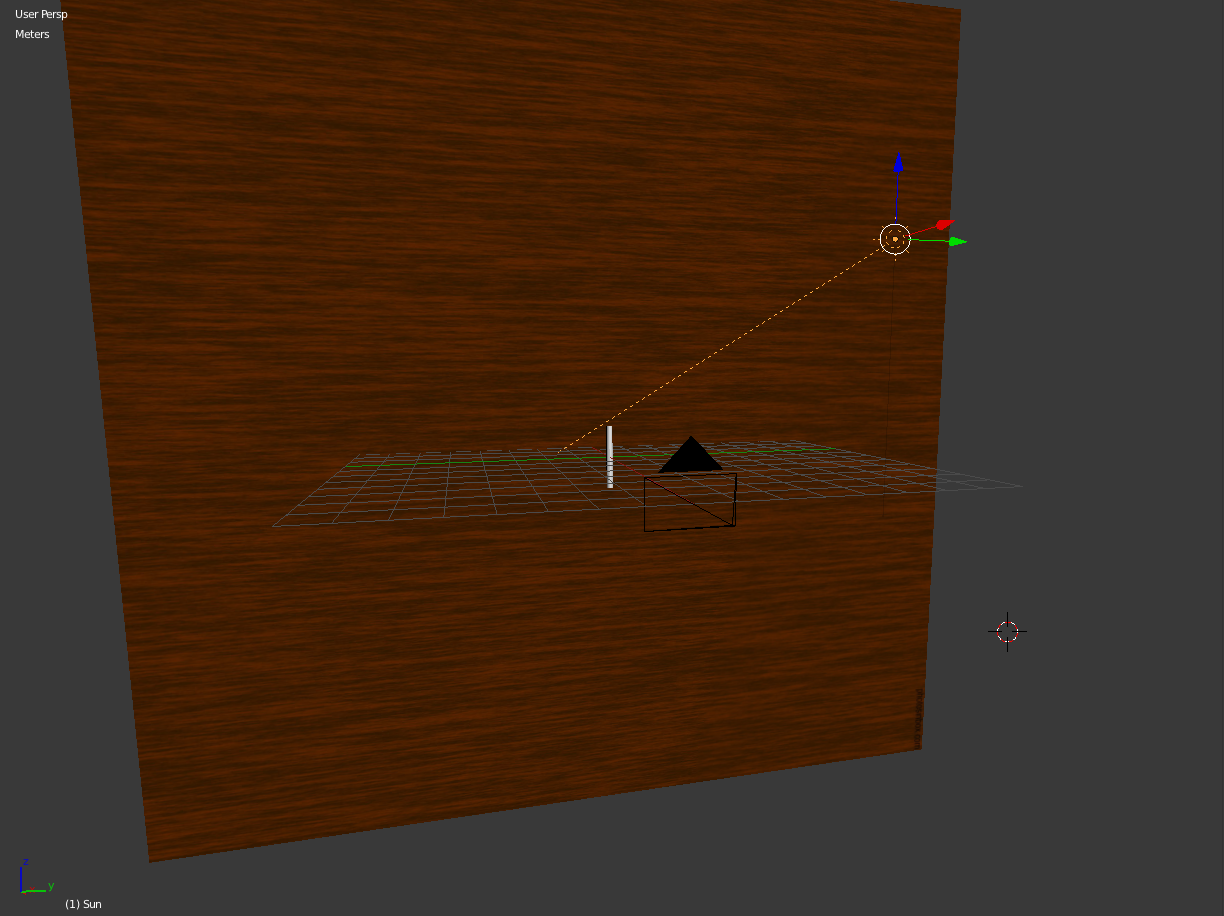
\includegraphics[width=\textwidth]{./Template_Figures/blender_scene}
        \caption{\label{fig:blender_scene}}
    \end{subfigure}
    \begin{subfigure}[b]{0.5\textwidth}
        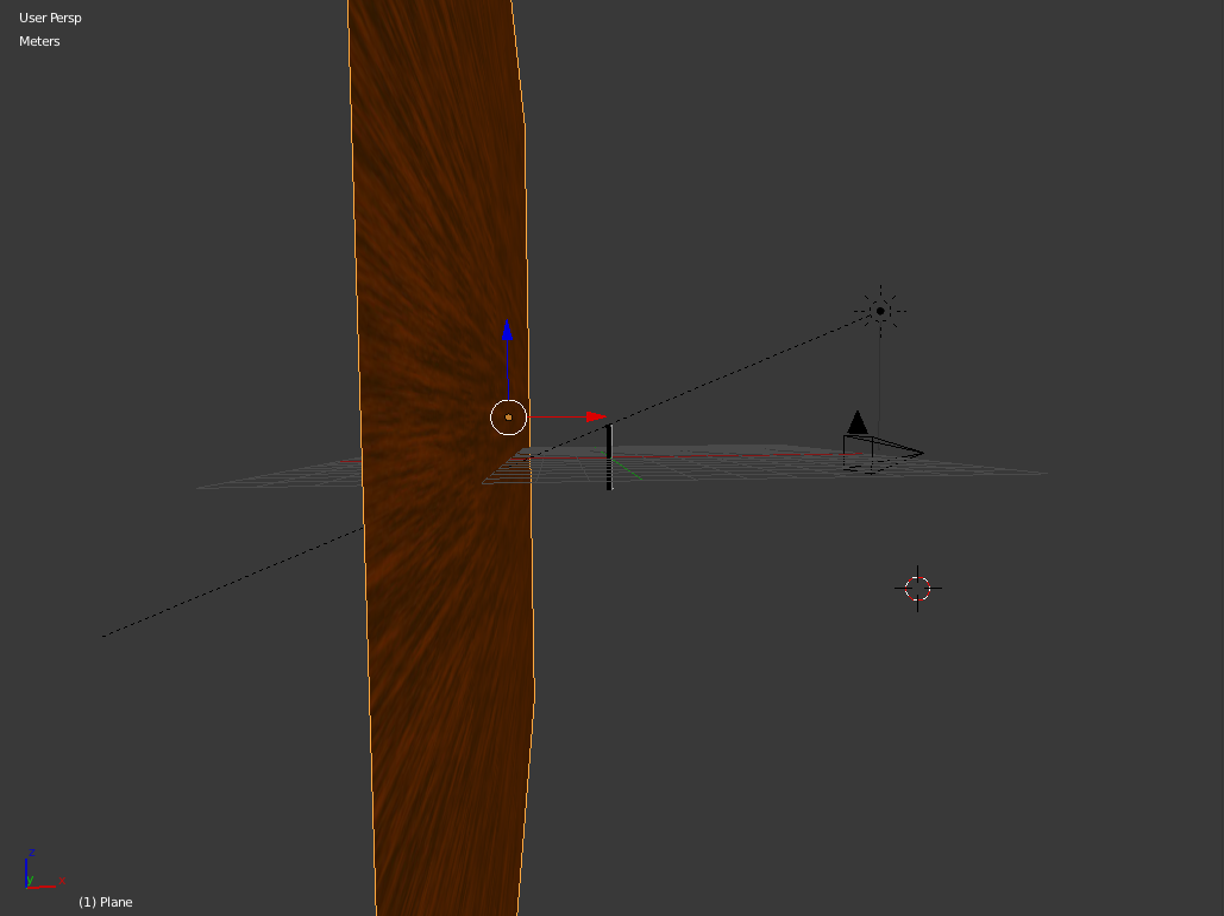
\includegraphics[width=\textwidth]{./Template_Figures/blender_scene_side}
        \caption{\label{fig:blender_scene_side}}
    \end{subfigure}
    \caption{(A) Frontal view of the scene rendered with Blender. (B) Side view of the same scene.\label{fig:Scene_conf}}
\end{figure}

In order to generate a set of stereo images with the object of interest at different disparities, the scene was captured with the camera baseline varying (in scene coordinates) between 0.2 cm and 12 cm with the step size of 0.2 cm. This gave us a set of 60 stereo images where the theoretical depth of the object of interest ranged from 0.04 cm to 3.45 cm (0 - 10.5 arc minutes in terms of crossed angular disparity) in front of the plane of focus (wooden plane). Figure \ref{fig:stimuli_stereo} shows stereo images of one of the cylinders and of the dragon. In a reference matching experiment, test subjects might use the discreet nature of the test stimulus as a matching cue. In order to avoid that, the step size was chosen small enough so that the transition from the minimum to the maximum depth for an object would seem continuous to the observer.
\begin{figure}[htbp]
    % \centering
    \begin{subfigure}[b]{0.5\textwidth}
        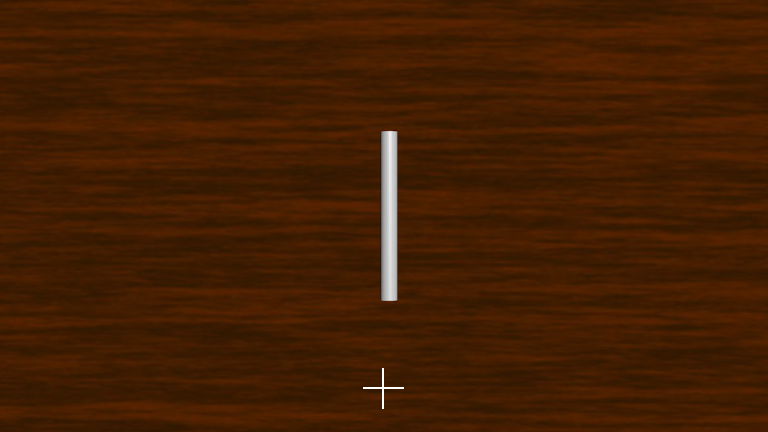
\includegraphics[width=\textwidth]{./Template_Figures/57L.png}
        \caption{}\label{fig:left_stereo_cyl}
    \end{subfigure}
    \begin{subfigure}[b]{0.5\textwidth}
        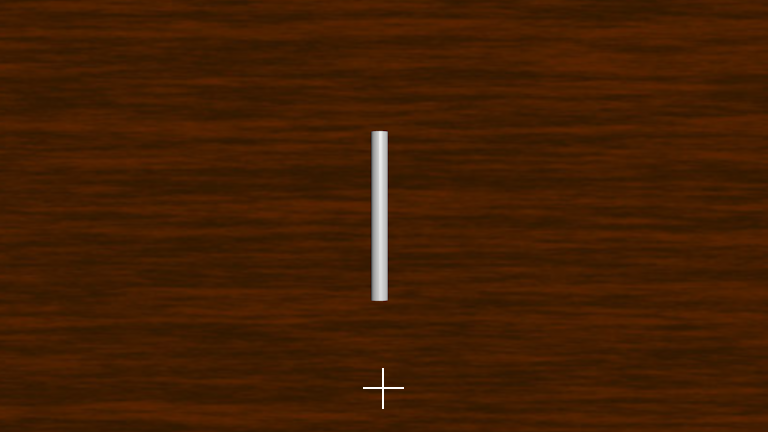
\includegraphics[width=\textwidth]{./Template_Figures/57R}
        \caption{}\label{fig:right_stereo_cyl}
    \end{subfigure}

    \begin{subfigure}[b]{0.5\textwidth}
        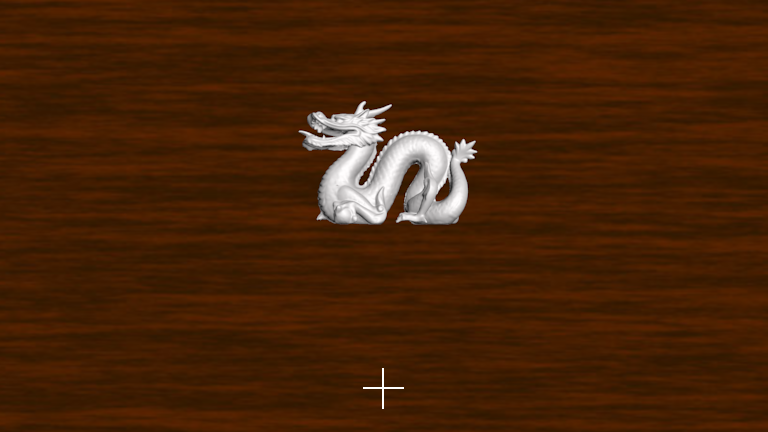
\includegraphics[width=\textwidth]{./Template_Figures/57Ld.png}
        \caption{}\label{fig:left_stereo_dra}
    \end{subfigure}
    \begin{subfigure}[b]{0.5\textwidth}
        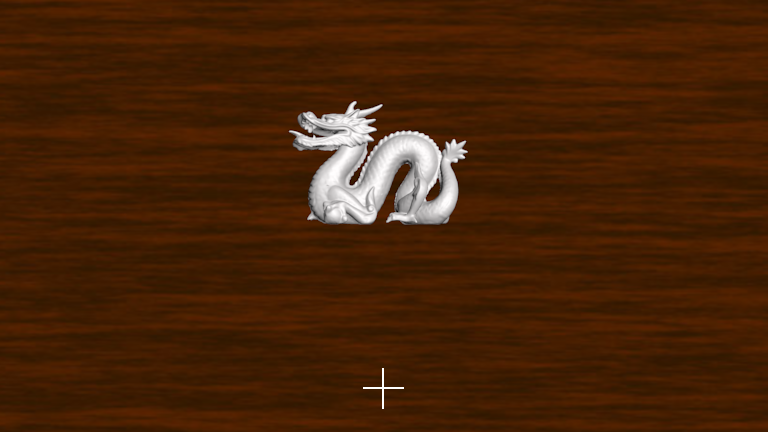
\includegraphics[width=\textwidth]{./Template_Figures/57Rd.png}
        \caption{}\label{fig:right_stereo_dra}
    \end{subfigure}
    \caption{Stereo images of the cylinder of 5 cm radius and the dragon. The theoretical depth difference between the objects and the background is 3.44 cm. Viewer can cross-fuse to see in depth.\label{fig:stimuli_stereo}}
\end{figure}

In order to compensate for symmetrical ghosts on both sides while the theoretical depth of object of interest remain unchanged, the images for automultiscopic experiments were rendered similarly with difference being that the range of baseline started from 0 cm until 24 cm. The reason for this is explained in the next section.

\section{Apparatus and simulation procedure}
The experiments were conducted on a commercial 47'' SIMS2 HDR47E LCD display with a spatial resolution of 1920$\times$1080. The left and right half of the screen each with a resolution of 960$\times$1080 were gated to the left and right eyes using a custom built Wheatstone setup \cite{ wiki:wheatstone} that consisted of two mirrors M1 and M2 set at a $45^\circ$ angle with respect to the screen. The optical length from the eyes to the screen via mirrors M1 and M2 was measured to be 87.3 cm. The whole setup was enclosed in a black box with an aperture through which the viewer could view the screen via mirrors M1 and M2. The display, even though built for HDR viewing had a \emph{DVI plus} mode for which the luminance measured with luminance meter via the aperture ranged from 0.47 $cd.m^{-2}$ to 1780 $cd.m^{-2}$. The \emph{DVI plus} mode should (according to the documentation) mimic a traditional LCD display, hence we chose to use this mode.
\begin{figure}[htbp]
    % \centering
    \begin{subfigure}[b]{0.5\textwidth}
        \includegraphics[width=\textwidth]{./Template_Figures/setup}
        \caption{}\label{fig:setup}
    \end{subfigure}
    \begin{subfigure}[b]{0.4\textwidth}
        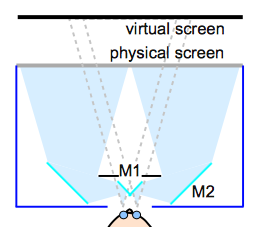
\includegraphics[width=\textwidth]{./Template_Figures/setup_sch}
        \caption{}\label{fig:setup_sch}
    \end{subfigure}
    \caption{(A) External view of our Wheatstone setup. (B) Internal schematics of the Wheatstone setup's enclosure box. Physical view frusta are shaded in light blue where as the virtual view frusta are depicted in dotted gray lines. The cyan lines represent the mirrors \cite{vangorp2014depth}.\label{fig:wheatstone_setup}}
\end{figure}

Since on an LCD panel, all the RGB channels equally and additively contribute to the crosstalk, we simulated the ghosted images simply by adding a percentage image of unintended view to the intended view image. For stereo, simple addition of a percentage of the right image into the left and vice versa sufficed. However, for the automultiscopic case, we simulated the view-luminance profiles (Figure \ref{fig:gaussians}) by fitting a Gaussian at each view. We found that an upscaled Gaussian such that it attains the value 0.8 at the mean ($\mu$) and with standard deviation ($\sigma$) = 2 matched the required view-luminance profile appropriately. Figure \ref{fig:sim_gaussians} shows 11 such Gaussians, the means ($\mu$) of whom are shifted according to the sweet spots of an 11-view automultiscopic display. Using our simulated profiles, we found that at any sweet spot viewing position, the amount of light leaked from views other then the two adjacent views can be considered as negligible. Hence, in our simulation we only considered light leakage from the two adjacent views. Figure \ref{fig:observed_ct_images} shows the simulated crosstalk on stereo and automultiscopic display. Considering that an automultiscopic screen displays light fields sampled at frequency $1/\delta_x$ ($\delta_x$ being the step size at which the images were captured along the camera baseline), the leaked light from a position `y' to position `x' can be modeled as:
\begin{equation}
l(y,x) \simeq a_y(x)\:.\:f(y)
\label{eq:ct_leak_eq}
\end{equation}
where $a_y(x)$ is the value of crosstalk as given by the Gaussian (corresponding to location \emph{y}) at position \emph{x}, and $f(y)$ is the light field image at position \emph{y}. The observed image \emph{g} at any viewing position \emph{x} can be mathematically modeled as:
\begin{equation}
g(x) \: \simeq \: ...\: +\: l(x-2\delta_x,\:x)\:+\: l(x-\delta_x,\:x)\:+\:l(x,\:x)\:+\: l(x+\delta_x,\:x)\:+\: l(x+2\delta_x,\:x)\:+ \:...
\label{eq:ct_sim_eq}
\end{equation}
This would mean that the amount of ghost separation at any disparity for an object would be constant on either side proportional to the object's parallax in $\delta_x$. In order to keep the nature of the automultiscopic experiments similar to that of the stereo (where the ghost separation increases as the disparity increases), we changed the sampling rate $\delta_x$ with respect to the disparity of the object. I.e., for a disparity \emph{2d}, the observed left and right images can be written as:
\begin{equation}
\begin{aligned}
g(d)_{left} \: \simeq l(2.d,\:d)\:+\: l(d,\:d)\:+\:l(0,\:d) \\
g(d)_{right} \: \simeq l(-2.d,\:-d)\:+\: l(-d,\:-d)\:+\:l(0,\:-d)
\end{aligned}
\label{eq:auto_obs_imgs}
\end{equation}

\begin{figure}
\centering
    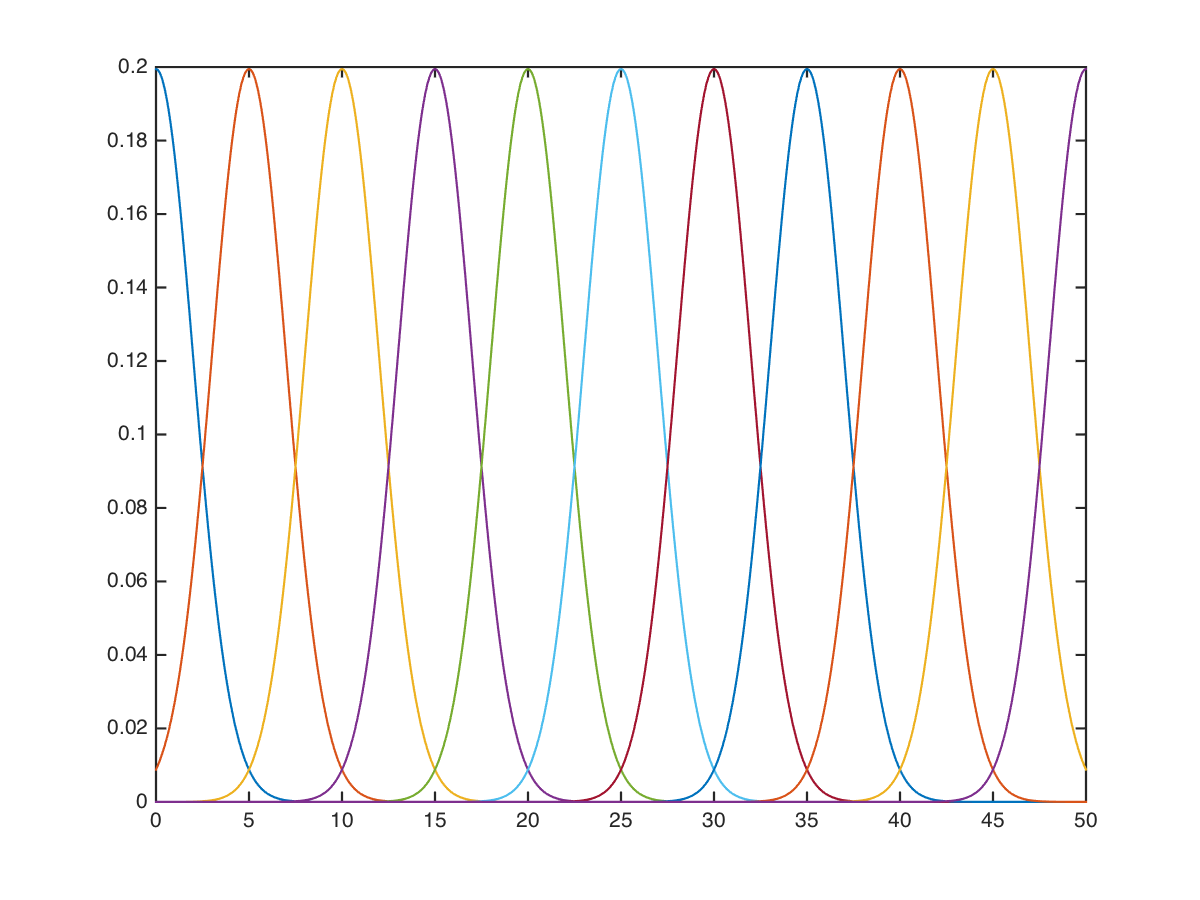
\includegraphics[width=0.7\textwidth]{./Template_Figures/sim_gaussians}
    \caption{View-luminance intensity profiles for an 11-view automultiscopic display simulated with Gaussians of $\sigma =2$ centered at the sweet spots. X-axis denote the viewing position. It can be seen that the simulated luminance profiles closely matches the experimentally observed view-luminance profiles in Figure \ref{fig:gaussians}\label{fig:sim_gaussians}}
\end{figure}

\begin{figure}[htbp]
    % \centering
    \begin{subfigure}[b]{0.5\textwidth}
        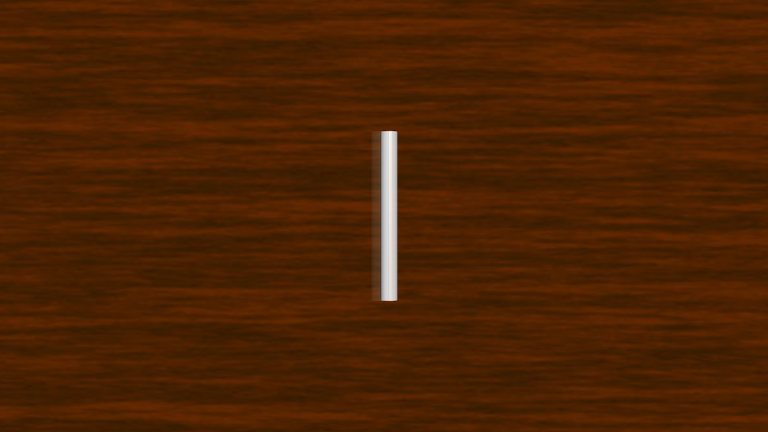
\includegraphics[width=\textwidth]{./Template_Figures/stereo_ghost_left}
        \caption{}\label{fig:obs_st_left}
    \end{subfigure}
    \begin{subfigure}[b]{0.5\textwidth}
        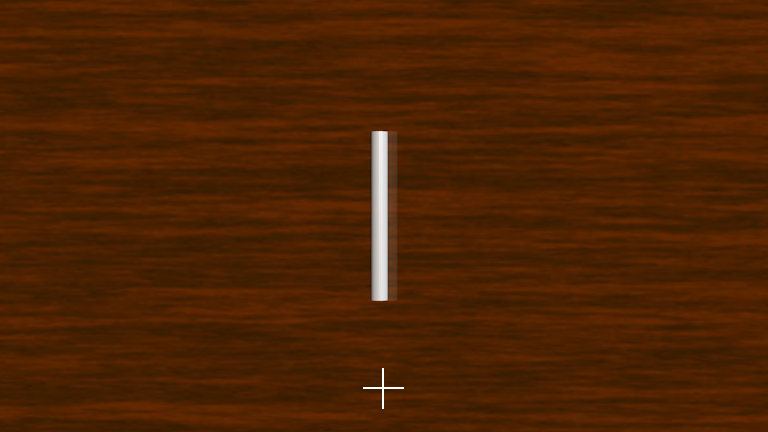
\includegraphics[width=\textwidth]{./Template_Figures/stereo_ghost_right}
        \caption{}\label{fig:obs_st_right}
    \end{subfigure}

    \begin{subfigure}[b]{0.5\textwidth}
        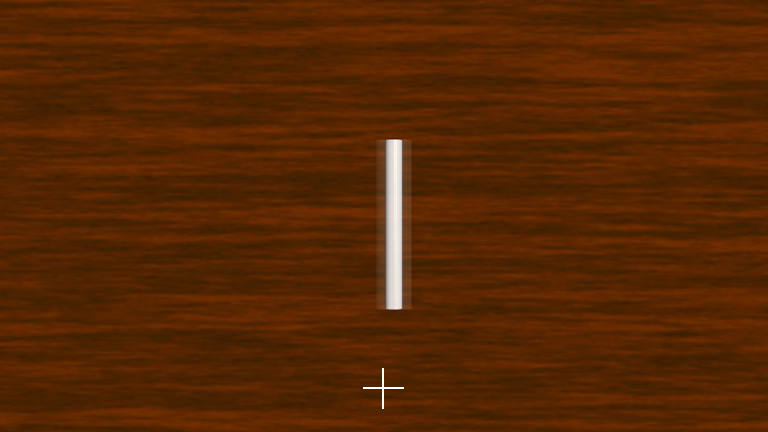
\includegraphics[width=\textwidth]{./Template_Figures/auto_ghost_left}
        \caption{}\label{fig:obs_aut_left}
    \end{subfigure}
    \begin{subfigure}[b]{0.5\textwidth}
        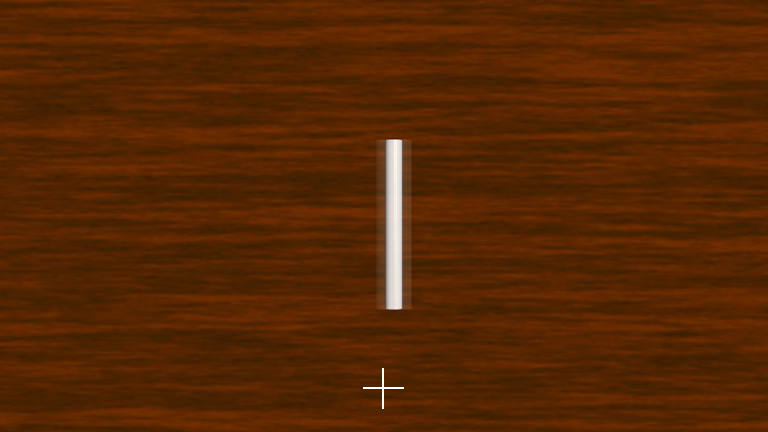
\includegraphics[width=\textwidth]{./Template_Figures/auto_ghost_left}
        \caption{}\label{fig:obs_aut_right}
    \end{subfigure}
    \caption{(a,b) Observed left and right stereo images containing 14\% crosstalk and crossed depth of 3.45 cm. (c,d) Same configuration for observed images on automultiscopic display. Viewers can cross-fuse to see in depth. Due to the fact that ghosting is not visible in the figure on printed document, viewers are encouraged to view this document in electronic form.\label{fig:observed_ct_images}}
\end{figure}

\section{Experimental procedure}
\subsection{Environment setup}
For our experiments, we subdivided the screen horizontally, i.e., the upper half, where the test subjects would see the crosstalk added stereo scene (stimuli) with some fixed depth of the object; and the lower half, where the subjects would see the same stereo scene without any added crosstalk. We will refer to the upper half of the screen as \emph{reference} stimulus and the lower half as \emph{test} stimulus. Also, we will call the depth difference between the background (wooden plane at zero disparity) and the foreground object (at some crossed disparity) as the depth of the stimulus (\emph{DoS})\index{DoS}. As mentioned in Section 4.2, \emph{DoS} in the presented stimuli ranged from 0.04 to 3.45 cm. The subjects could vary \emph{DoS} in the test stimulus in the above mentioned range via left and right mouse buttons. Due to the dense sampling of the light field (small baseline distance change between stimuli), the change in the depth appeared continuous, i.e., the viewers could not observe any jumps while changing it. Pressing the left mouse button continuously for 6 seconds would change the  \emph{DoS} from 0.04 cm to 3.45 cm, and vice versa for the right mouse button. The subjects could stop anywhere in between by releasing the mouse button. During the experiment, the subjects were tasked with matching the \emph{DoS} in the test stimulus to the \emph{DoS} of the reference stimulus. Upon matching \emph{DoS}, the subjects would register the answer using the center mouse button. Figure \ref{fig:exp_env} shows the overall layout of the screen from a viewer's perspective. To avoid the possibility of the subject matching the absolute depths of the objects in stimuli rather than \emph{DoS}, as required, we shifted the global depth of the reference stimulus by 3.45 cm away from the screen depth (towards the viewer) whereas the global depth of the test stimulus was shifted equally and similarly away from the viewer. We thus ensured that the absolute depths of the objects in stimuli would never coincide, and hence, the subjects would not be able to, and would not attempt to match the absolute object's depth. In order to make this arrangement obvious to the viewer, a nonious cross-hair representing the plane of focus (located at the depth of the physical screen) was added at the bottom center of the screen. Figure \ref{fig:exp_env_depth} shows the top view of the visualized environment. The experiment environment was created using the Psychtoolbox-3 package for Matlab, which was also used to record the subject's answers.
\begin{figure}[htbp]
    \centering
    \begin{subfigure}[b]{0.8\textwidth}
        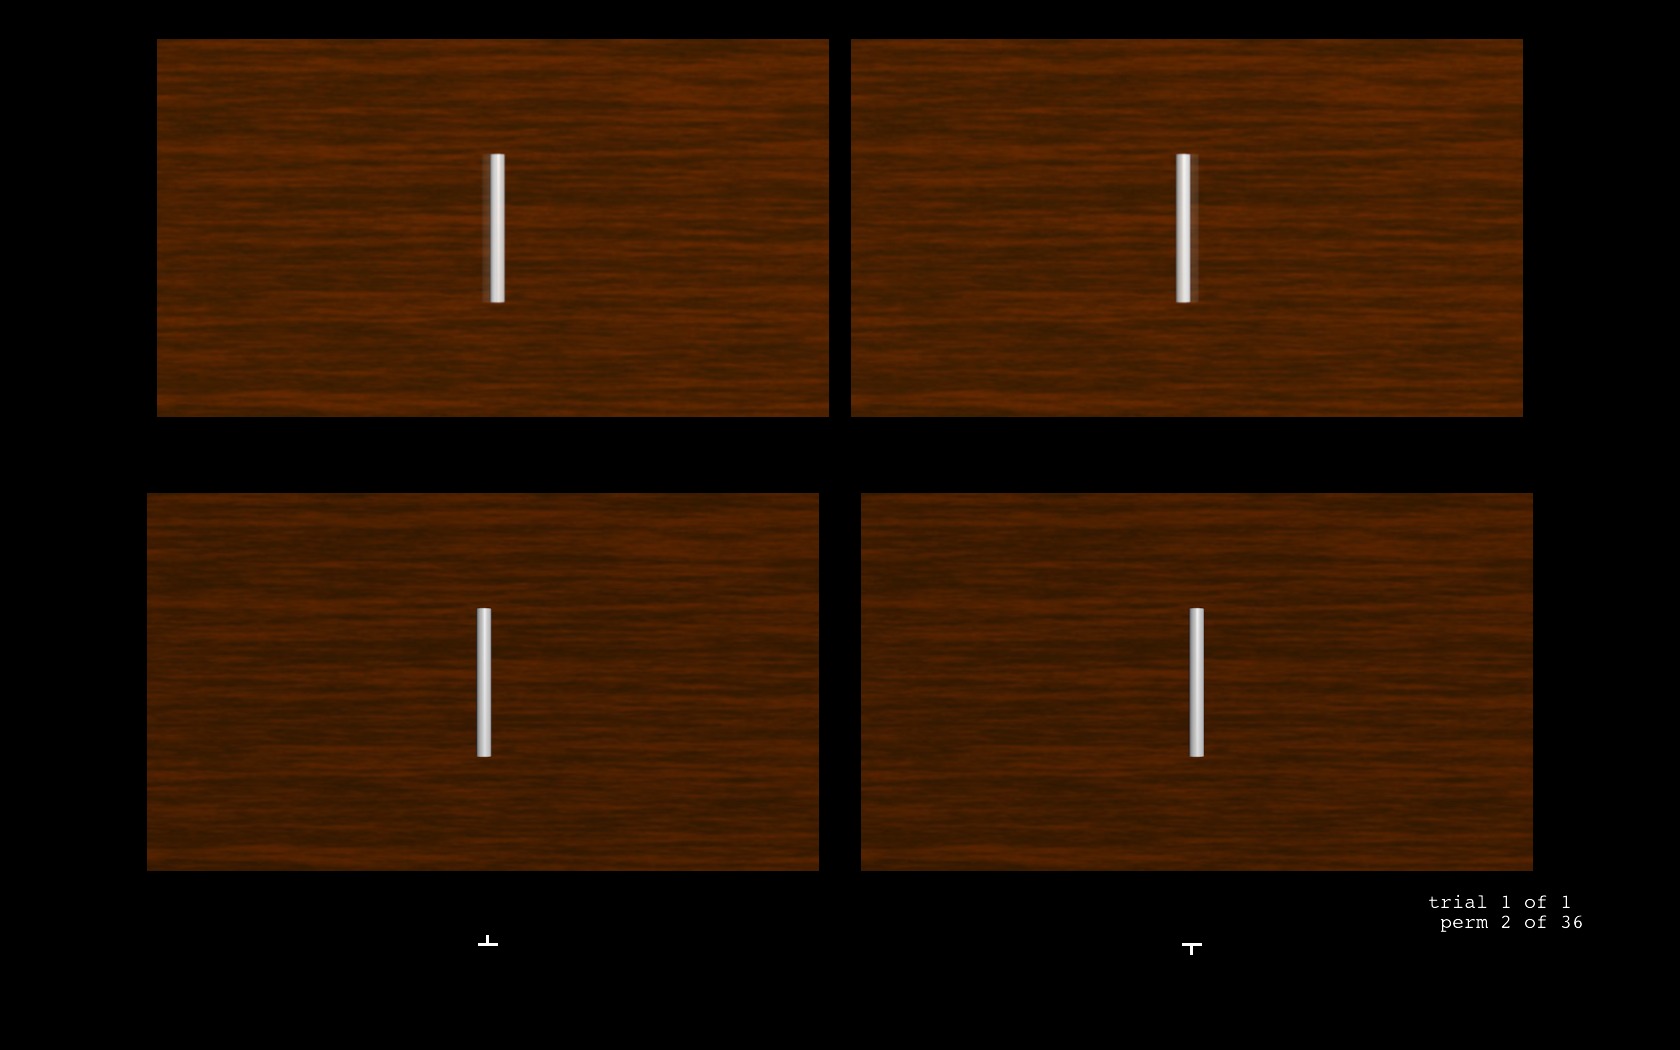
\includegraphics[width=\textwidth]{./Template_Figures/exp_env}
        \caption{}\label{fig:exp_env}
    \end{subfigure}

    \begin{subfigure}[b]{0.4\textwidth}
        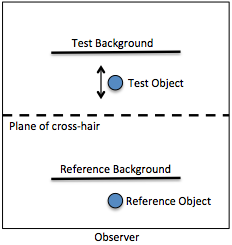
\includegraphics[width=\textwidth]{./Template_Figures/exp_env_depth}
        \caption{}\label{fig:exp_env_depth}
    \end{subfigure}

    \caption{(A) Schematics of the complete display. Upper half of the screen shows the reference stimulus, in this case, with 14\% crosstalk. The bottom half shows the user-controlled test stimulus which is always free of crosstalk. (B) Layout of the experiment environment in terms of depth w.r.t. observer. Due to the fact that ghosting is not visible in the figure on printed document, viewers are encouraged to view this document in electronic form.\label{fig:exp_env_overall}}
\end{figure}

\subsection{Subjects}
Several paid test subjects and the author participated in the experiments. In order to ensure subject's correctness of the stereo vision, they were first asked to identify the proximity of the test and reference stimuli with respect to the cross-hair. Then they were asked to identify the polarity of the change in depth of the test stimulus while the author changed it slightly in each direction randomly. Table \ref{tab:agg_subj} shows the number of participants in each kind of experiment.
\begin{table}[ht!]
  \begin{center}
    \caption{Number of subjects that participated in each experiment.}
    \label{tab:agg_subj}
    \begin{tabular}{ccc}
      \toprule
      Object & Stereo  & Automultiscopic\\
      \midrule
      Cylinder(thin) & 11 & 13  \\
      Cylinder(medium) & 11 & 11\\
      Cylinder(thick) & 7 & 13\\
      Cylinder(thickest) & 8 & 13 \\
      Dragon & 13 & 13\\
      \bottomrule
    \end{tabular}
  \end{center}
\end{table}

\subsection{Experiment parameters}
Four levels of crosstalk (0\%, 3\%, 7\% and 14\%) and seven levels of DoS (crossed disparity of object) (0.04, 0.73, 1.18, 1.53, 1.75, 2.76 and 3.44 cm) were chosen to be tested. We neglected any level of crosstalk greater than 14\% because in our pilot experiments we noticed that any greater crosstalk level almost always led to matching of the stimulus with the ghost, instead of the corresponding stimulus, resulting in total loss of depth. Further we could not find any commercial stereo display where the crosstalk levels were that high: Usually they are below 10\%. During the experiment, each subject was asked to match the observed depths for the 28 possible combinations (4 crosstalk levels $\times$ 7 DoS levels) for each kind of stimulus. Trials for stereoscopic and automultiscopic cases were conducted separately.
\\
\section{Results}

In this section, we show the results obtained for the different experiments performed. In all cases, we show the median data for all the observers along with the standard error for each crosstalk level, DoS and geometry (Figure \ref{fig:s_crosstalk_0} to Figure \ref{fig:a_crosstalk_14}). Individual lines in the graphs denote the different objects used as stimuli (See Table \ref{tab:stimili_desc}). The \emph{x} and \emph{y} axis denotes the actual (theoretical) and the viewer-observed depths of the stimuli respectively. Ideally, if crosstalk had no effect on the perceived depth, all the graphs should be diagonally coinciding lines. Even though generally this is not the case, it can be observed that in the base case (no crosstalk), all the graphs, for all objects, almost approximates a diagonal line for both stereo and automultiscopic experiments. This is an improvement over \cite{tsirlin2012effect} meaning that the reported amounts of depth degradation for different cases would be more reliable, since in our case, the base case (0\% crosstalk) is consistent with what previous literature reports \cite{palmisano2010stereoscopic}.

\subsection{Stereoscopic case}
It can be seen in Figure \ref{fig:s_crosstalk_0} that in the absence of crosstalk, observers mostly perceived depths correctly. A slight overestimation of depth in case of the smallest depth (0.04 cm) can be seen for the thickest cylinder (width = 36 arc min). Given the fact that the user-controlled depth variation of the test stimulus was continuous, it is reasonable to assume that it would be quite unlikely for the observers to exactly match the depths. Hence the slight overestimation of depth can be considered as an observer approximation error. The same, however, could not be straightforwardly said about the underestimation for the dragon at 2.76 cm depth which is mapped to approximately 2 cm observed depth. But since the next greater depth shows no underestimation, we can safely assume it to be a human error.
\begin{figure}[H]
\centering
    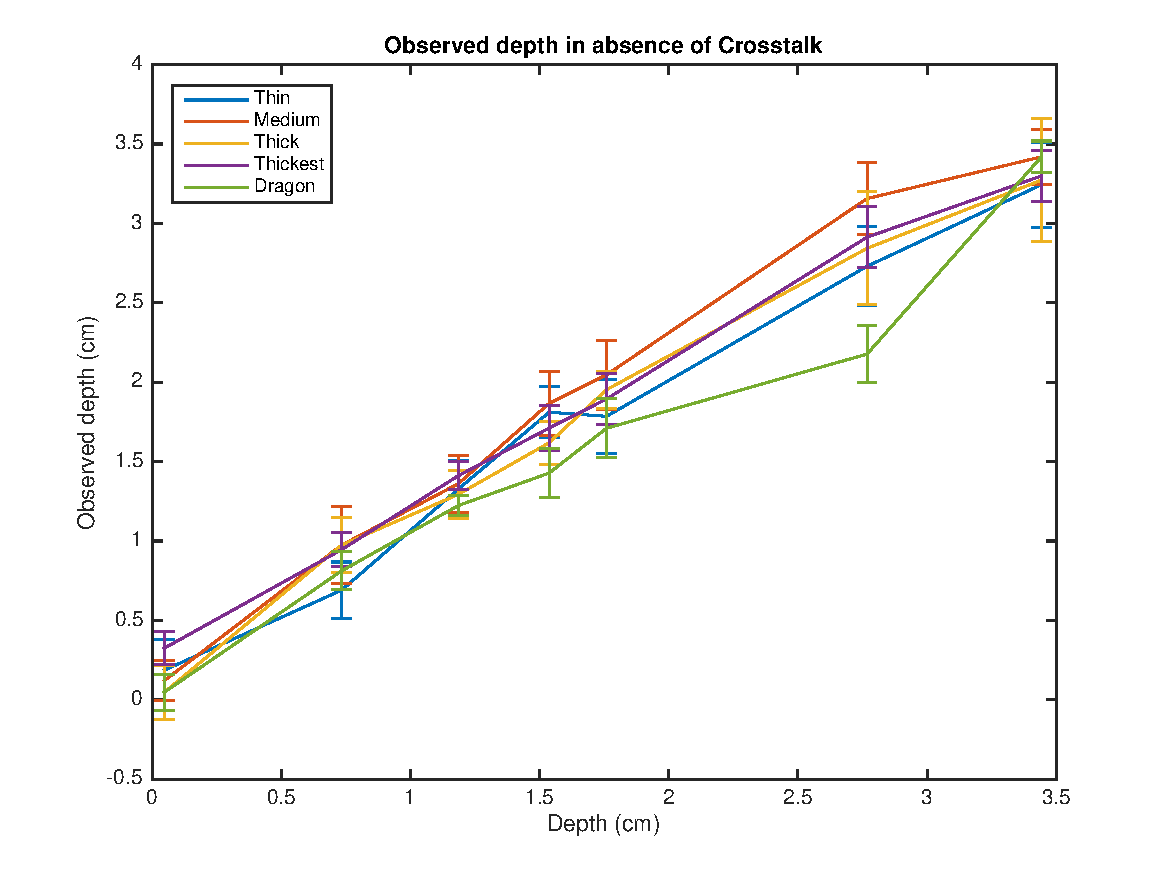
\includegraphics[width=0.9\textwidth]{./Template_Figures/s_crosstalk_0}
    \caption{The median data for all observers is shown. The abscissa shows the observed depth when no crosstalk is present, in comparison with the theoretical depth. Different lines represent different stimuli. The error bars indicate $\pm$ 1 standard error.\label{fig:s_crosstalk_0}}
\end{figure}

When the crosstalk is increased to 3\% (Figure \ref{fig:s_crosstalk_3}), it is clear that the observed depth of the thin (18.9 arc min) cylinder starts degrading at depths greater than 1.75 cm. The angular disparity at this depth is 5.35 arc min which would give a ghost separation\footnote{Ghost separation is defined as the percentage of ghost stimulus that does not spatially overlap the stimulus.} of 28\%. A slight overestimation of the 2.76 cm depth for the thickest cylinder (75.6 arc min) can be considered as approximation error, since the next greater depth is observed without any degradation. We think it would be reasonable to consider this as a human approximation error because the HVS probably does not gets confused for some disparity and then behaves without any error for the following larger disparities. I.e. Once the observed depth starts degrading at some disparity, provided all the other conditions are kept constant, it should keep on degrading for all larger disparities as well.
\begin{figure}[H]
\centering
    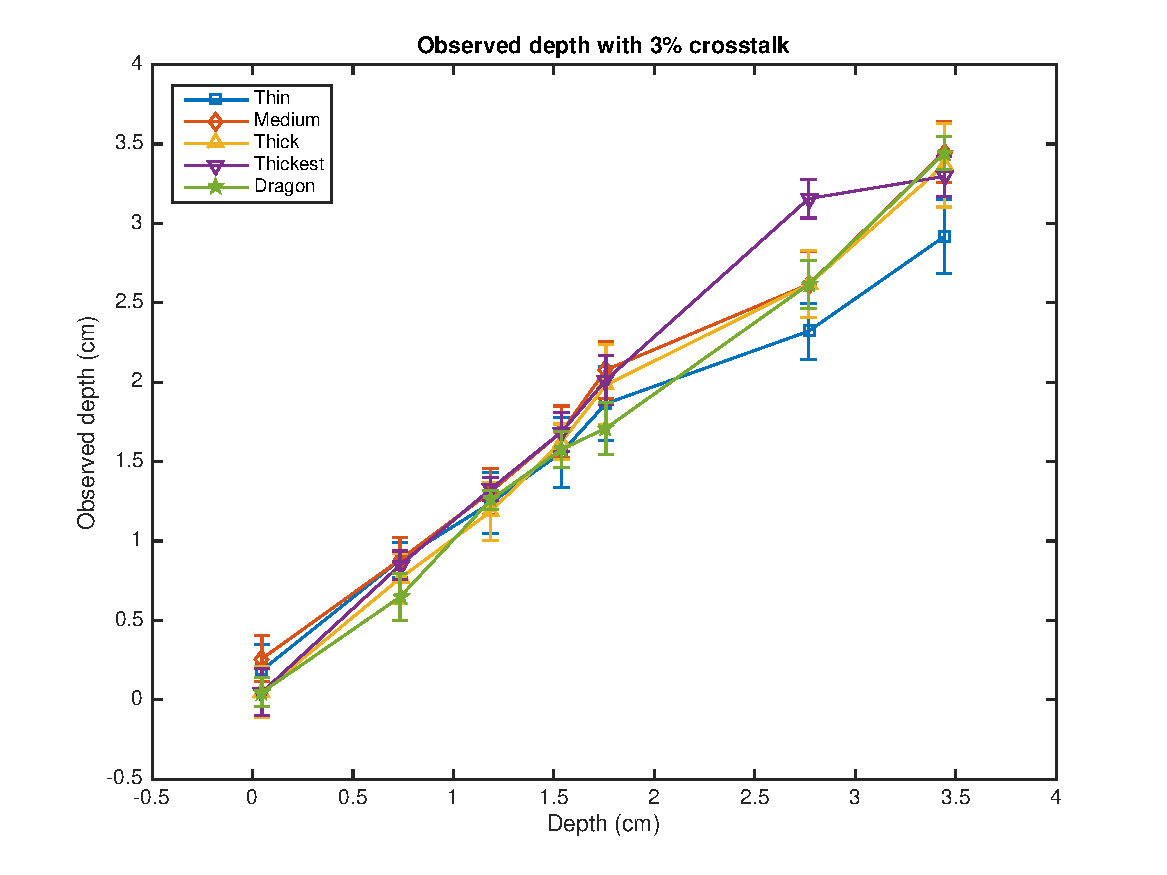
\includegraphics[width=0.9\textwidth]{./Template_Figures/s_crosstalk_3}
    \caption{The median data for all observers is shown. The abscissa shows the observed depth when 3\% crosstalk is present, in comparison with the theoretical depth. Different lines represent different stimuli. The error bars indicate $\pm$ 1 standard error.\label{fig:s_crosstalk_3}}
\end{figure}

Substantial effects on the observed depth start appearing once the crosstalk level is increased to 7\% (see Figure \ref{fig:s_crosstalk_7}). The cylinders of all widths show reduced observed depth. The reduction is most severe for the thin (18.9 arc min) cylinder. The loss of observed depth appears to be lower as the width of the cylinder increases while the observed depth of the dragon seems to be unaffected. One interesting point to observe is that for all the cylinders, the perceived depth starts degrading at the actual depths of 1.75 cm or higher. For the thin cylinder, the ghost is completely separated only at the maximum depth i.e., 3.45 cm. However the observed depth appears to be the same for the maximum and the second maximum i.e. 2.76 cm depth. Also it should be noted that the graph for the thin cylinder shows signs of degradation even at a depth of 1.13 cm.

Observed depth is severely affected for all the object once the crosstalk reaches 14\% (see Figure \ref{fig:s_crosstalk_14}). The thin cylinder again shows signs of degradation starting at a depth of 1.13 cm where as the observed depths of all the other objects start deteriorating at the theoretical depth of 1.76 cm. The pattern of wider objects showing less depth deterioration compared to thin objects is still observed. However, with such extreme crosstalk level, even the observed depth of the dragon is reported to be substantially affected.

\begin{figure}[H]
\centering
    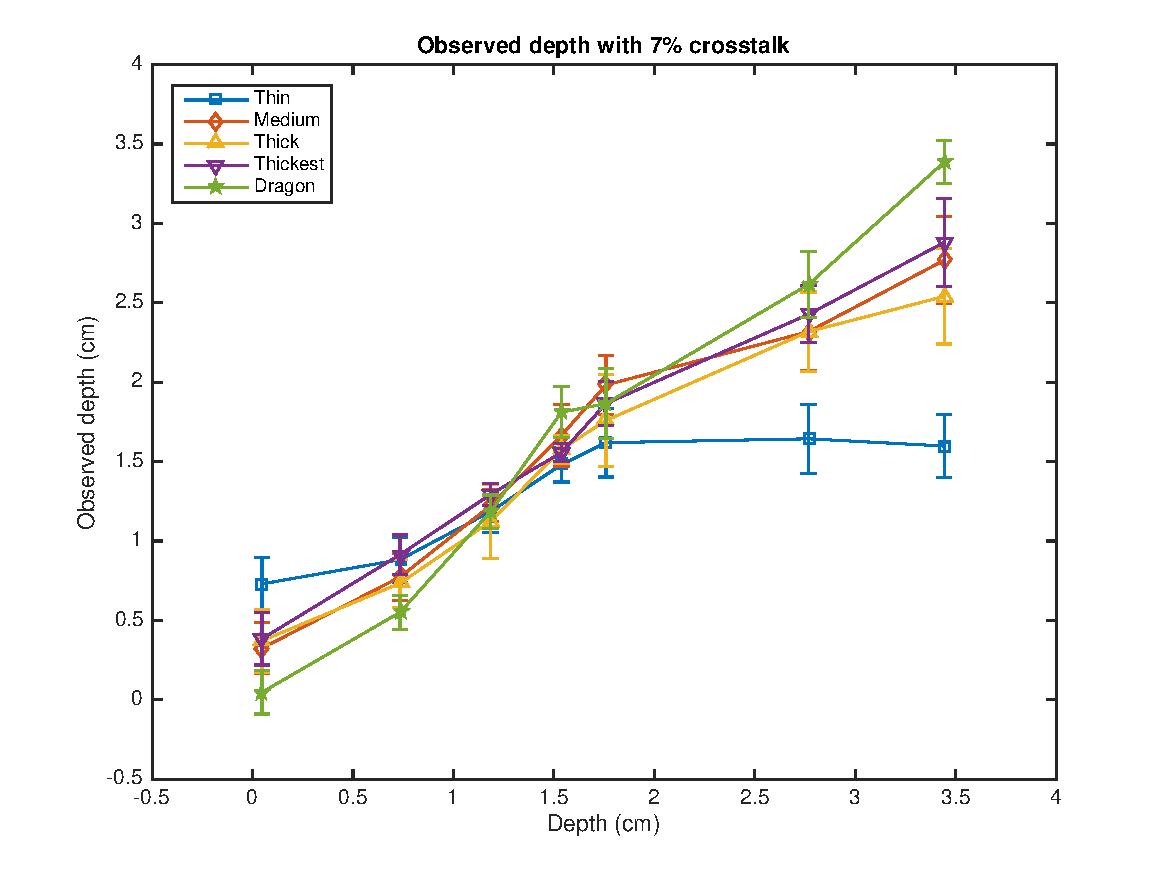
\includegraphics[width=0.9\textwidth]{./Template_Figures/s_crosstalk_7}
    \caption{The median data for all observers is shown. The abscissa shows the observed depth when 7\% crosstalk is present, in comparison with the theoretical depth. Different lines represent different stimuli. The error bars indicate $\pm$ 1 standard error.\label{fig:s_crosstalk_7}}
\end{figure}

\begin{figure}[H]
\centering
    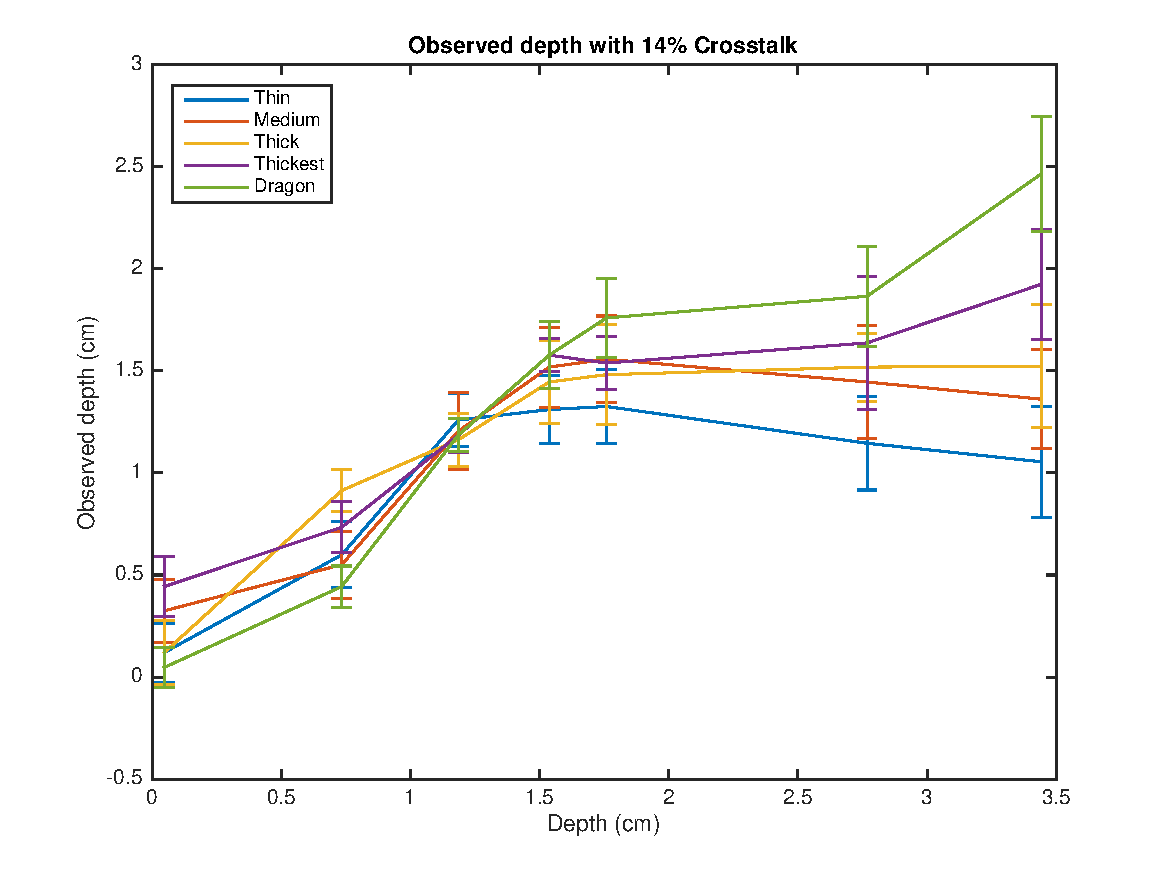
\includegraphics[width=0.9\textwidth]{./Template_Figures/s_crosstalk_14}
\caption{The median data for all observers is shown. The abscissa shows the observed depth when 14\% crosstalk is present, in comparison with the theoretical depth. Different lines represent different stimuli. The error bars indicate $\pm$ 1 standard error.\label{fig:s_crosstalk_14}}
\end{figure}



\subsection{Automultiscopic case}


Figure \ref{fig:a_crosstalk_0} shows the pattern of the observed depth in the base case (i.e., 0\% crosstalk). It appears that the observed depth for the dragon is slightly overestimated at the actual depth of 2.76 cm. At the same instance, the observed depth of the thick cylinder is underestimated. These exceptional cases may be considered again as human error, firstly because the next greater depth is observed without any error and secondly because this case is exactly the same as the base case of the stereo experiments. However, the fact that there is mostly (both stereo and automultiscopic case) some mis-judgment of the depth may also indicate that the HVS for some reason is being confused by this particular depth.

We notice that the crosstalk has no effect on the perceived depth when the crosstalk level is raised to 3\% (Figure \ref{fig:a_crosstalk_3}). This is because for each of the perceived depth, the base case observed depth is in the rage of the standard error. This is different than the stereoscopic scenario where we observed some minute depth reduction for the thin cylinder. Increasing the crosstalk to 7\% (Figure \ref{fig:a_crosstalk_7}) however, shows signs of degraded depth for the medium (37.8 arc min) cylinder depths larger than 2.76 cm. Meanwhile all the other objects show no evidence of degraded depth even though the crosstalk level at 7\% is higher than what we usually get from a conventional automultiscopic display \cite{woods2012crosstalk}.
\begin{figure}[H]
\centering
    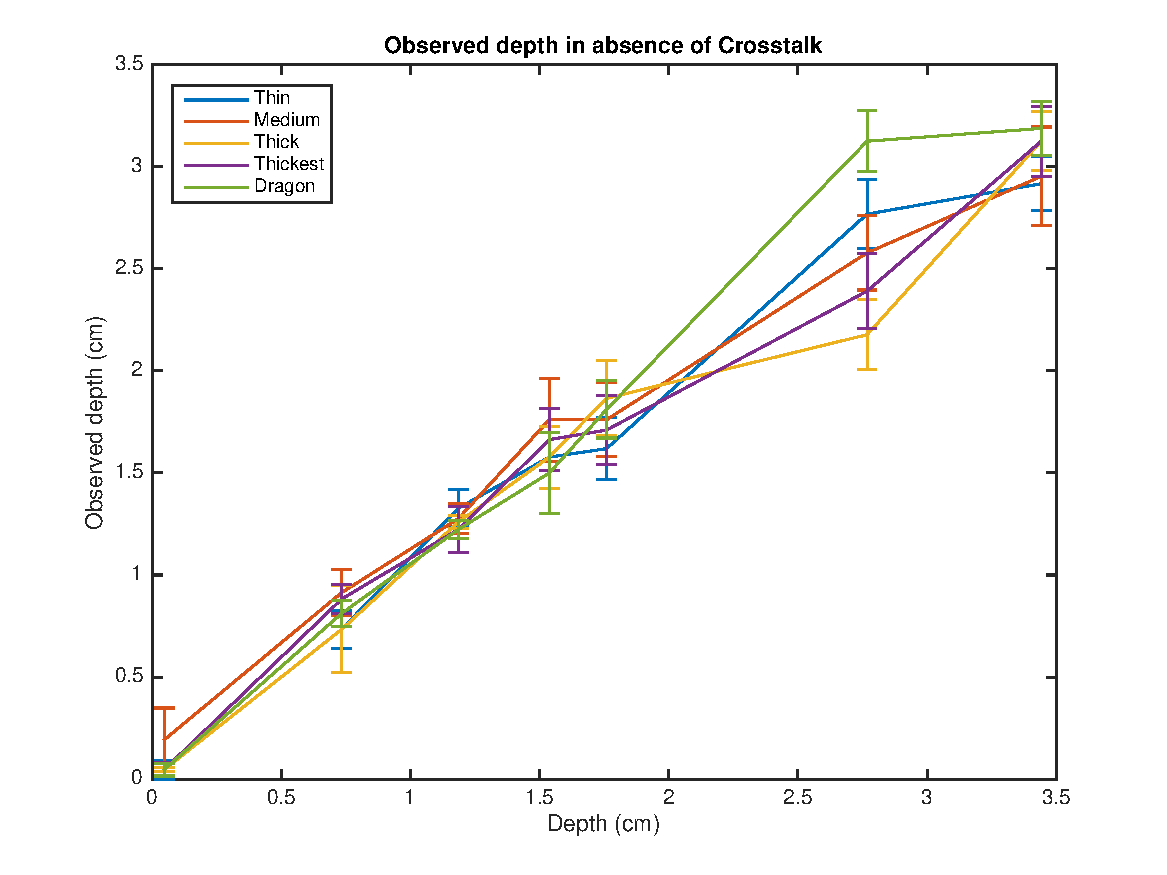
\includegraphics[width=0.9\textwidth]{./Template_Figures/a_crosstalk_0}
    \caption{The median data for all observers is shown. The abscissa shows the observed depth when no crosstalk is present, in comparison with the theoretical depth. Different lines represent different stimuli. The error bars indicate $\pm$ 1 standard error.\label{fig:a_crosstalk_0}}
\end{figure}

\begin{figure}[H]
\centering
    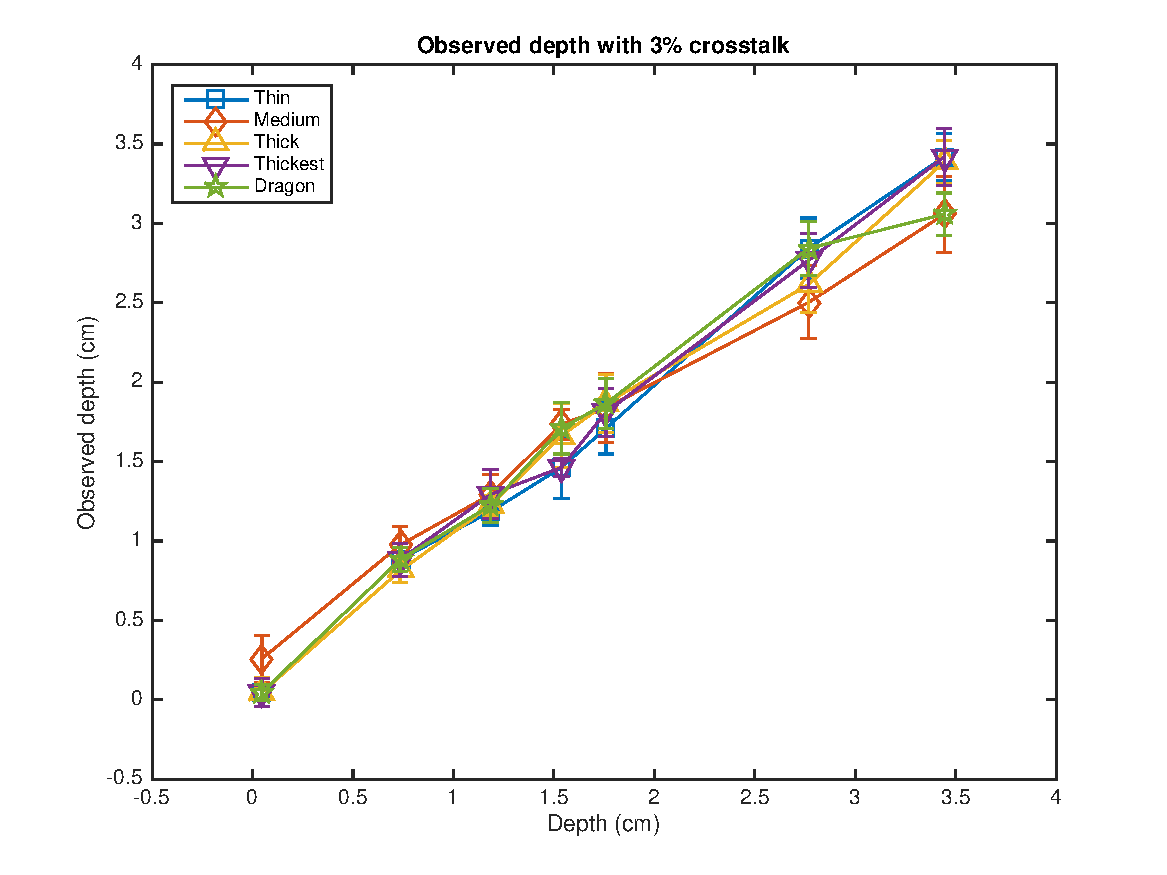
\includegraphics[width=0.9\textwidth]{./Template_Figures/a_crosstalk_3}
    \caption{The median data for all observers is shown. The abscissa shows the observed depth when 3\% crosstalk is present, in comparison with the theoretical depth. Different lines represent different stimuli. The error bars indicate $\pm$ 1 standard error.\label{fig:a_crosstalk_3}}
\end{figure}

\begin{figure}[H]
\centering
    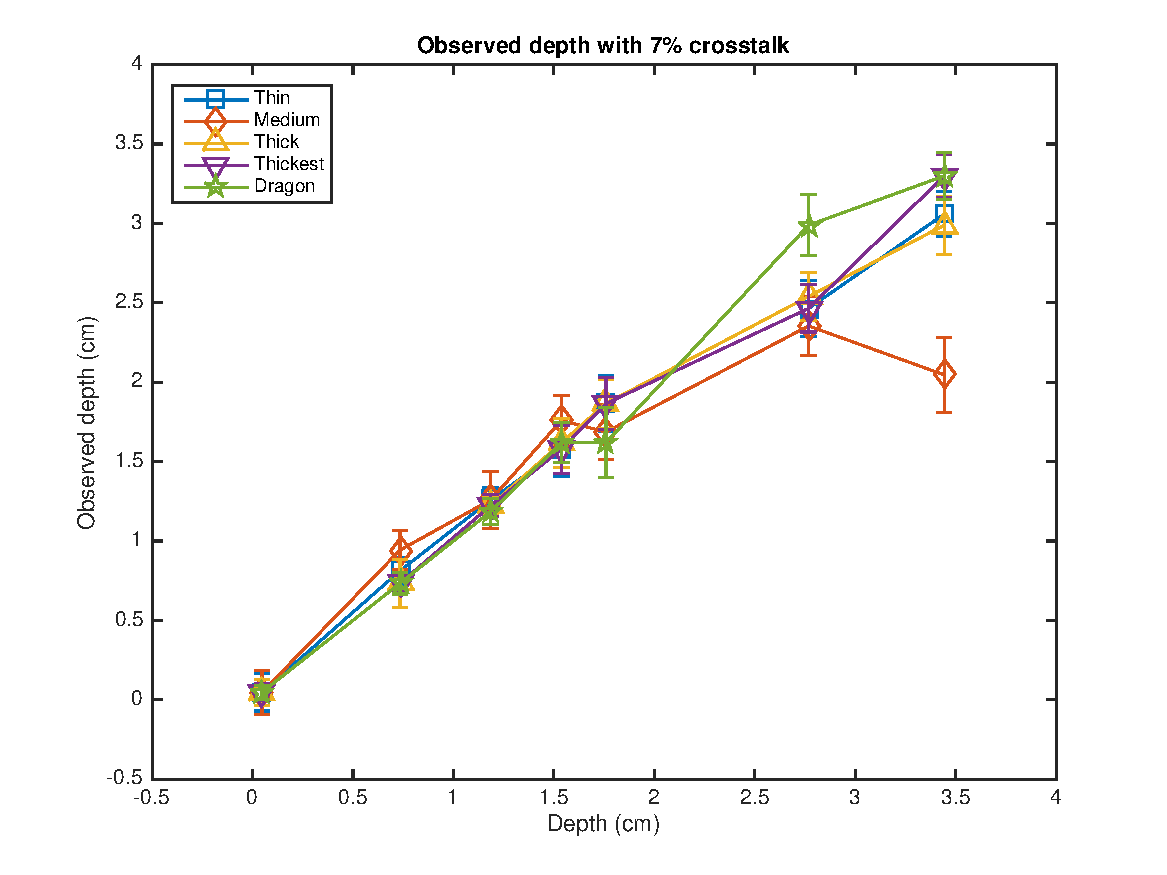
\includegraphics[width=0.9\textwidth]{./Template_Figures/a_crosstalk_7}
    \caption{The median data for all observers is shown. The abscissa shows the observed depth when 7\% crosstalk is present, in comparison with the theoretical depth. Different lines represent different stimuli. The error bars indicate $\pm$ 1 standard error.\label{fig:a_crosstalk_7}}
\end{figure}

\begin{figure}[H]
\centering
    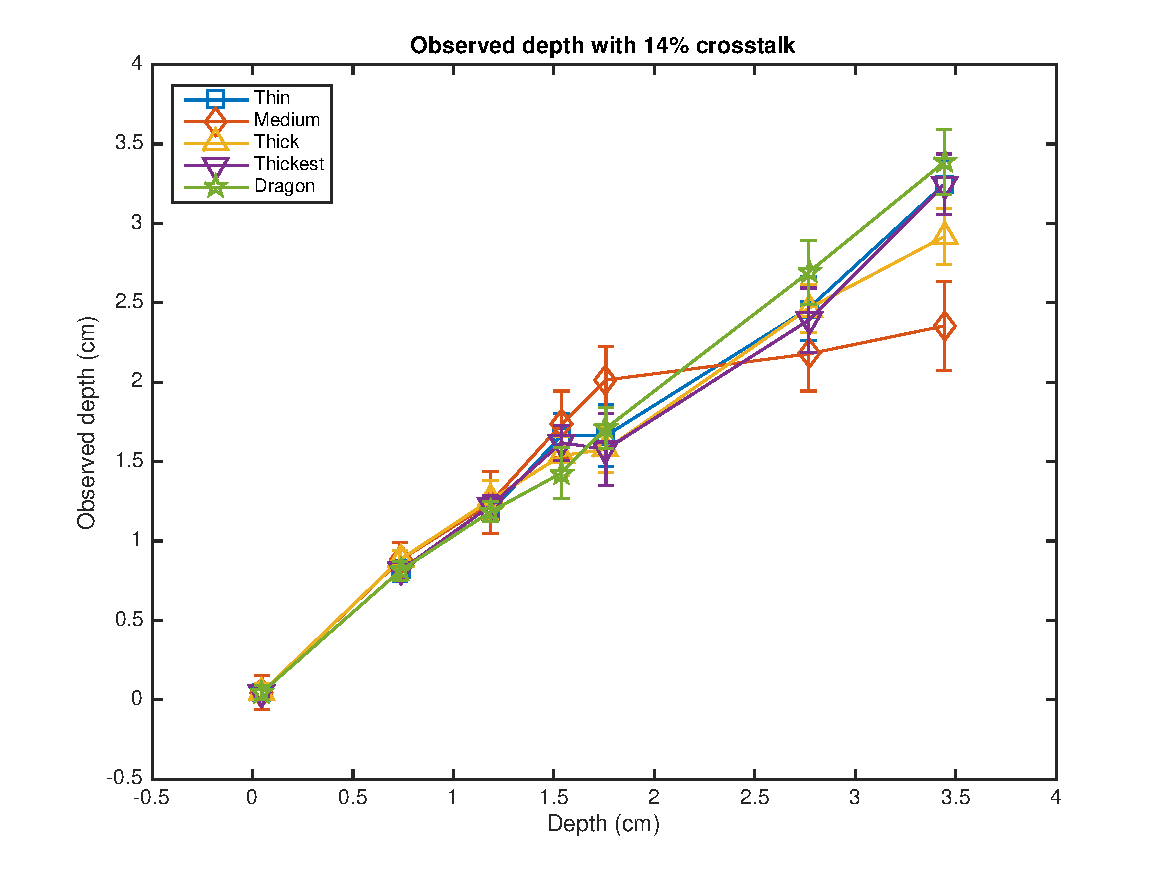
\includegraphics[width=0.9\textwidth]{./Template_Figures/a_crosstalk_14}
    \caption{The median data for all observers is shown. The abscissa shows the observed depth when 14\% crosstalk is present, in comparison with the theoretical depth. Different lines represent different stimuli. The error bars indicate $\pm$ 1 standard error.\label{fig:a_crosstalk_14}}
\end{figure}
Interestingly, increasing the crosstalk level to 14\% also shows that for most cases, the perceived depth is not different than the depth observed in absence of crosstalk. It is not clear why only the medium cylinder shows depth degradation in this case. However, based on the results it is clear that the effect of crosstalk on the perceived depth is significantly lower (or negligible) in the automultiscopic environment. Possible explanations for all these behaviors can be found in the next section.

\section {Discussion}
\subsection{Stereoscopic case}
%Explain what we have observed?
In these experiments, we found that for the stereoscopic case, crosstalk has a substantial degrading effect on the magnitude of perceived depth. The perceived depth magnitude relative to the 0\% crosstalk base case deceases as the crosstalk level increases. Moreover, for a fixed value of crosstalk, the degradation effect seems to be more pronounced as the disparity increases. This effect is stronger on the thin objects as compared to the wider ones. One of our initial hypothesis suggesting that the perceived depth magnitude might not be degraded once the ghost and the object separate completely (i.e. no overlap between them) was also proven to be wrong as the results clearly show degradation even in the those cases. In order to explain these results, we have to delve into the theories regarding how the HVS extracts depth from disparity.

There is evidence to suggest that the HVS uses the cross-correlation between horizontally displaced patches on the two retinal images to obtain the disparity of objects \cite{filippini2009limits}\cite{kane2014limits}. The disparity, once the cross-correlation is performed, is extracted by locating the peaks in the resultant correlation profiles \cite{cormack1991interocular}. It is easier for the HVS to identify clear sharp peaks compared to broad noisy ones as shown in Figure \ref{fig:cormack}. Since adding crosstalk additively to an image effectively reduces the global contrast and severely reduces the local contrast around the object, it is obvious that the HVS will have more difficulty in resolving the proper disparity, a possible reason for the observed depth degradation. Also it is believed that the patches chosen for interocular cross-correlation are filtered by two dimensional isotropic Gaussians (Gaussian windows) \cite{filippini2009limits}. It is not clear what the size (constant or variable) of those windows is.

If the HVS could somehow match the patch containing the ghost-object pair in one retinal image to the other, then according to windowed cross-correlation theory, because there would be no ambiguity, disparity computed would either be zero or the actual disparity without any degradation. However, we think that the HVS in case of stereo only uses the object-containing patch in one retinal image to obtain the horizontal disparity based on correlation with the other image. One of the reasons for this is that HVS has a certain limitation and it cannot fuse two objects together if the disparity gradient (defined as the ratio of disparity difference between two objects and their cyclopean angular separation) is greater than 1-1.5 \cite{howard1995binocular} \cite{kane2014limits}. In case of stereo pairs, where the objects in both images have a crossed disparity, their ghosts have an equally uncrossed disparity relative to the plane of focus. This, in terms of geometry, is only possible if the ghost is located exactly behind the object (similar to the double nail illusion as illustrated in \cite{tsirlin2012effect} \cite{krol1980double}) making the disparity gradient $\infty$. In such cases, the stimulus with higher luminance (the actual object) is fused leaving the ghost in diplopic state. The other reason is that the HVS also takes into consideration the polarity of the luminance changes between patches in order to find a correct match. This means that an object whose left side is black and right side is white will not be matched to the object in the corresponding retinal image who's left side is white and right side is black \cite{howard1995binocular}. In case of stereoscopy with added crosstalk, the polarity of the ghost-object luminance change in one retinal image is the opposite of the other. Hence it is reasonable to assume that a patch that only contains the object of interest from one retinal image is chosen to compute the horizontal interocular cross-correlation with the other. We tried simulating the disparity estimation via interocular cross-correlation using the model proposed in \cite{filippini2009limits} and found that the crosstalk had no effect on the computed disparity.

For the x, y position of an object in one of the stereo images, the ghost in the other image is present at the exact same location while the actual object is located at some horizontal disparity \emph{d}. Computing the cross-correlation in this case would result in two distinct peaks, one at zero disparity and the other at disparity \emph{d}. Hence the HVS might apply some averaging in order to obtain a disparity. This, however, is only possible when the disparity is large enough to separate the ghost from the object completely. As seen in Figure \ref{fig:normal_ccr}, this is not the case when the ghost is not fully separated from the object. In this case the correlation will result in one peak. Considering the correlation profile, we observe that there is difference between the slope around zero disparity (location of the ghost) and the actual disparity \emph{d}. It is known \cite{howard1995binocular} that the HVS also uses the first derivative of luminance in order to find matching portions of stereo images. In that case, the HVS can still isolate two distinct peaks in the cross-correlation profile where one peak results at zero disparity, representing maximum correlation with the ghost, and the other at disparity \emph{d}, representing the maximum correlation with the object. Since the HVS gives preference to lower disparities \cite{krol1980double}, if the averaging is performed based on the heights and the distances (relative to the zero disparity) of the peaks, then this might explain the loss of perceived depth magnitude that is proportional to the crosstalk level. This would also explain why at some crosstalk level threshold (16\% in our experiments), the ghosts are matched to the original objects and the viewer perceives two copies of the object side by side (double nail illusion \cite{tsirlin2012effect}) located at the plane of focus. However, this will still not explain why wider objects result in lower loss of perceived depth magnitude as compared to thin objects.

In our experiment, we also noticed that the perceived depth magnitude remains unaffected for some small disparities even when the crosstalk level is at 14\%. For 3\% crosstalk, this threshold is the angular disparity of 5.25 arc min (1.75 cm depth) where as, for the crosstalk levels of 7\% and 14\%, these thresholds seem to be 4.2 arc min (1.5 cm) and 3.15 arc min (1.18 cm) respectively. This suggests that the HVS probably does not average the disparities at locations of interocular cross-correlation peaks as that would have resulted in a degraded perceived depth at every disparity. Our proposed modified windowed interocular cross-correlation model explained in chapter 5 might explain these results.

Our results are consistent with the current literature and show a clear degrading effect on the perceived depth that increases with the increase of crosstalk level and the decrease of object's width. Kooi et al \cite{kooi2004visual} showed that as low as 5\% crosstalk can result in reduced visual comfort. Considering that and based on our results, we recommend that the crosstalk levels in stereoscopic 3D displays should not exceed more than 3\%. At this level we found that the perceived depth is not significantly degraded for stimuli of any shape or geometry. \pagebreak


\subsection{Automultiscopic case}

At first impression, one might hypothesize that the crosstalk should have a greater effect on the observed depth in automultiscopic scenes for the simple reason that the number of ghosts per image is greater (at least one on each side of the object as opposed to only one ghost in case of stereo). Our results however, indicate that there was no substantial effect of crosstalk on the perceived depth magnitude in automultiscopic environment. We believe that the HVS in case of automultiscopic environment, given the existing symmetry, matches the patches containing the tuple (left-ghost, object and right-ghost) in one retinal image to the similarly appearing patch in the other one. One reason for this as mentioned in the previous section is that the HVS considers the polarity of luminance changes in the object. The tuples in both the retinal images have the same luminance profiles. The other reason is that matching the tuples containing patching in this way will not violate any disparity gradient which was the case with the ghosts in stereoscopic environment.

\begin{table}[ht!]
  \begin{center}
    \caption{Ghosts and objects seen in an automultiscopic environment according to Equation \ref{eq:auto_obs_imgs}}
    \label{tab:ghost_obj_names}
    \begin{tabular}{ccc}
      \toprule
      Image & Stimulus  & Location(disparity)\\
      \midrule
                       & Left ghost & 0  \\
      Left eye image   & Object & $\frac{d}{2}$\\
                       & Right ghost & $d$\\
                       &             & \\
                       & Left ghost & $-d$  \\
      Right eye image  & Object & $-\frac{d}{2}$\\
                       & Right ghost & 0\\
      \bottomrule
    \end{tabular}
  \end{center}
\end{table}

It can be seen from Table \ref{tab:ghost_obj_names} that the tuple appearing in the left eye is located at a disparity \emph{d} in the right eye image. And since matching tuple containing patches will not cause any confusion (due to disparity gradient violation etc), it is clear why the viewers were able to report the proper depths (in most cases) for the objects despite of raising the crosstalk level to 14\%. Based on our results we can conclude that crosstalk does not have any significant effect on the observed depth in automultiscopic displays. However, since the number of ghosts are twice the amount found in stereoscopic screens, we can predict that crosstalk in automultiscopic screen may affect the viewers visual comfort to a greater extent. Our experiments simulated only for the sweet spot of an automultiscopic screens. It should be noted that even though amount of light leakage from neighboring views will change as the viewer moves away from the sweet spot, the pattern of the luminance changes throughout the objects will remain the same. Hence, the observed depths of the objects will not be affected. The observed geometry of the objects with complex geometry however might change (depending on the scene) due to crosstalk if the viewer is not located at the sweet spots.

Given the fact that the amount of crosstalk changes as the viewer moves his/her viewing position, and the fact that crosstalk might change the observed geometry of the objects in the scene while viewing from a non-sweet spot position, it is difficult to recommend a minimum level of crosstalk that ensures a pleasant and comfortable viewing experience. We know that as low as 5\% of crosstalk in a stereoscopic display is enough to result in visual discomfort. We can predict that this threshold would be much lower for an automultiscopic display. However, further research must be carried out in order to provide such objective measurements. In particular, future work should focus on analyzing the crosstalk effects of depth perception on both complex and non complex stimuli for viewers located outside the sweet spot. In this work, what we did establish, for the first time, is the absence of a significant effect of crosstalk on perceived depth magnitude in the case of automultiscopic displays, which is different to what happens in stereoscopic displays.

\begin{table}[ht!]
  \begin{center}
    \caption{Insert Caption}
    \label{tab:posthoc_stereo}
    \begin{tabular}{cccccccc}
      \toprule
      \specialcell{Sample\\crosstalk\\(\%)} & \specialcell{Depth \\(cm)} & \specialcell{p-val \\(thin)} & \specialcell{p-val \\(medium)} & \specialcell{p-val \\(thick)} & \specialcell{p-val \\(thickest)} & \specialcell{p-val \\(dragon)}\\
      \midrule
         3 & 0.047     & 0.24121                     & 0.39337                   & 0.54688                   & 0.53125           & 0.8125 \\
           & 0.734      & 0.48582                     & 0.12127                   & 0.37573                   & 0.083984          & 0.25 \\
           & 1.185       & 0.60121                     & 0.30024                   & 0.21631                   & 0.37573           & 0.36646 \\
           & 1.537       & 0.20433                     & 0.22279                   & 0.30127                   & 0.80774           & 0.33936 \\
           & 1.759        & 0.45527                     & 0.73795                   & 0.6355                    & 0.71484           & 0.7334 \\
           & 2.767       & 0.013005                    & 0.069337                  & 0.89258                   & 0.032715          & 0.083984 \\
           & 3.442        & 0.10046                     & 0.76272                   & 0.50159                   & 0.66956           & 0.76953 \\
         7 & 0.047     & 0.032742                    & 0.17098                   & 0.23047                   & 0.054688          & 0.5625 \\
           & 0.734      & 0.62739                     & 0.028828                  & 0.13086                   & 0.32031           & 0.27832 \\
           & 1.185       & 0.72098                     & 0.0081426                 & 0.32581                   & 0.4126            & 0.46973 \\
           & 1.537       & 0.00090225                  & 0.31731                   & 1                         & 0.26758           & 0.092285 \\
           & 1.759        & 0.4455                      & 0.073565                  & 0.063965                  & 0.7334            & 0.89258 \\
           & 2.767       & 0.00090225                  & 0.036104                  & 0.42627                   & 0.078491          & 0.55664 \\
           & 3.442        & 0.0057843                   & 0.0055762                 & 0.026611                  & 0.26758           & 0.22266 \\
        14 & 0.047     & 0.54163                     & 0.098889                  & 0.94531                   & 0.13086           & 0.21875 \\
           & 0.734      & 0.15308                     & 0.0072316                 & 0.68481                   & 0.026855          & 0.0058594 \\
           & 1.185       & 0.064149           & 0.0063133                 & 0.42627                   & 0.003418          & 1 \\
           & 1.537       & 0.00010642         & 0.029885                  & 0.1394                    & 0.00097656        & 0.98242 \\
           & 1.759        & 0.018585           & 2.0983e-05                & 0.080322                  & 0.013184          & 0.79102 \\
           & 2.767       & 7.9941e-05         & 0.00013216                & 0.005249                  & 0.00085449        & 0.2334 \\
           & 3.442        & 0.00033392         & 1.6676e-05                & 0.00048828                & 0.00048828        & 0.054688 \\
      \bottomrule
    \end{tabular}
  \end{center}
\end{table}

\begin{table}[ht!]
  \begin{center}
    \caption{Insert Caption}
    \label{tab:posthoc_stereo_null}
    \begin{tabular}{cccccccc}
      \toprule
      \specialcell{Sample\\crosstalk\\(\%)} & \specialcell{Depth \\(cm)} & \specialcell{Hypothesis\\rejection \\(thin)} & \specialcell{Hypothesis\\rejection \\(medium)} & \specialcell{Hypothesis\\rejection \\(thick)} & \specialcell{Hypothesis\\rejection \\(thickest)} & \specialcell{Hypothesis\\rejection \\(dragon)}\\
      \midrule
           3&                   0.047&           0        &           0        &           0        &           0        &           0  \\      
            &                    0.734&           0        &           0        &           0        &           0        &           0     \\   
            &                    1.185&           0        &           0        &           0        &           0        &           0        \\
            &                     1.537&           0        &           0        &           0        &           0        &           0        \\
            &                     1.759&           0        &           0        &           0        &           0        &           0        \\
            &                   2.767&           1        &           0        &           0        &           1        &           0        \\
            &               3.442&           0        &           0        &           0        &           0        &           0        \\
           7&                   0.047&           1        &           0        &           0        &           0        &           0       \\ 
            &                  0.734&           0        &           1        &           0        &           0        &           0        \\
            &                1.185&           0        &           1        &           0        &           0        &           0        \\
            &                    1.537&           1        &           0        &           0        &           0        &           0        \\
            &                   1.759&           0        &           0        &           0        &           0        &           0        \\
            &                    2.767&           1        &           1        &           0        &           0        &           0        \\
            &                    3.442&           1        &           1        &           1        &           0        &           0        \\
          14&                   0.047&           0        &           0        &           0        &           0        &           0       \\ 
            &           0.734&           0        &           1        &           0        &           1        &           1        \\
            &          1.185&           0        &           1        &           0        &           1        &           0        \\
            &           1.537&           1        &           1        &           0        &           1        &           0        \\
            &           1.759&           1        &           1        &           0        &           1        &           0        \\
            &          2.767&           1        &           1        &           1        &           1        &           0        \\
            &          3.442&           1        &           1        &           1        &           1        &           0        \\
      \bottomrule
    \end{tabular}
  \end{center}
\end{table}







\begin{table}[ht!]
  \begin{center}
    \caption{Posthoc auto}
    \label{tab:posthoc_auto}
    \begin{tabular}{cccccccc}
      \toprule
      \specialcell{Sample\\crosstalk\\(\%)} & \specialcell{Depth \\(cm)} & \specialcell{p-val \\(thin)} & \specialcell{p-val \\(medium)} & \specialcell{p-val \\(thick)} & \specialcell{p-val \\(thickest)} & \specialcell{p-val \\(dragon)}\\
      \midrule
   3&          0.047&          0.8125&          0.5719&          0.03125&          1&          0.5 \\
    &          0.734&          0.3396&          0.1454&          0.94604&          0.83105&          0.62207 \\
    &          1.185&          0.10986&          0.90953&          0.375&          0.16016&          0.3396 \\
    &          1.537&          0.37573&          0.29588&          0.67725&          0.077148&          0.56934 \\
    &          1.759&          1&          0.34106&          1&          0.19678&          1 \\
    &          2.767&          1&          0.23044&          0.15137&          0.36646&          0.38037 \\
    &          3.442&          0.26611&          0.33916&          0.27832&          0.41309&          0.51855 \\
   7&          0.047&          1&          0.056152&          0.25&          0.34375&          0.625 \\
    &          0.734&          0.79102&          0.9133&          0.68481&          0.08374&          0.5625 \\
    &          1.185&          1&          0.48124&          0.41431&          0.77539&          0.89844 \\
    &          1.537&          0.2334&          0.2891&          0.55664&          0.41309&          0.62207 \\
    &          1.759&          0.49731&          0.091845&          0.42383&          0.73438&          0.73535 \\
    &          2.767&          0.38037&          0.83287&          0.1748&          0.8501&          0.45117 \\
    &          3.442&          0.74951&          0.02497&          0.45483&          0.30127&          0.83105 \\
  14&          0.047&          0.51563&          0.0031738&          0.09375&          1&          0.25 \\
    &          0.734&          0.28809&          0.67907&          0.38501&          0.027344&          0.26587 \\
    &          1.185&          0.080322&          0.68485&          0.95215&          0.96191&          0.86475 \\
    &          1.537&          0.57715&          0.74125&          0.49731&          0.62207&          0.33936 \\
    &          1.759&          0.90723&          0.23047&          0.12939&          0.78687&          0.56934 \\
    &          2.767&          0.36523&          0.40774&          0.12305&          0.96973&          0.12305 \\
    &          3.442&          0.46484&          0.21724&          0.25&          0.7002&          0.7002 \\
      \bottomrule
    \end{tabular}
  \end{center}
\end{table}

\begin{table}[ht!]
  \begin{center}
    \caption{Posthoc auto null}
    \label{tab:posthoc_auto_null}
    \begin{tabular}{cccccccc}
      \toprule
      \specialcell{Sample\\crosstalk\\(\%)} & \specialcell{Depth \\(cm)} & \specialcell{Hypothesis\\rejection \\(thin)} & \specialcell{Hypothesis\\rejection \\(medium)} & \specialcell{Hypothesis\\rejection \\(thick)} & \specialcell{Hypothesis\\rejection \\(thickest)} & \specialcell{Hypothesis\\rejection \\(dragon)}\\
      \midrule
   3      &       0.047      &       0      &       0      &       1      &       0      &       0 \\
          &       0.734      &       0      &       0      &       0      &       0      &       0 \\
          &       1.185      &       0      &       0      &       0      &       0      &       0 \\
          &       1.537      &       0      &       0      &       0      &       0      &       0 \\
          &       1.759      &       0      &       0      &       0      &       0      &       0 \\
          &       2.767      &       0      &       0      &       0      &       0      &       0 \\
          &       3.442      &       0      &       0      &       0      &       0      &       0 \\
   7      &       0.047      &       0      &       0      &       0      &       0      &       0 \\
          &       0.734      &       0      &       0      &       0      &       0      &       0 \\
          &       1.185      &       0      &       0      &       0      &       0      &       0 \\
          &       1.537      &       0      &       0      &       0      &       0      &       0 \\
          &       1.759      &       0      &       0      &       0      &       0      &       0 \\
          &       2.767      &       0      &       0      &       0      &       0      &       0 \\
          &       3.442      &       0      &       1      &       0      &       0      &       0 \\
  14      &       0.047      &       0      &       1      &       0      &       0      &       0 \\
          &       0.734      &       0      &       0      &       0      &       1      &       0 \\
          &       1.185      &       0      &       0      &       0      &       0      &       0 \\ 
          &       1.537      &       0      &       0      &       0      &       0      &       0 \\
          &       1.759      &       0      &       0      &       0      &       0      &       0 \\
          &       2.767      &       0      &       0      &       0      &       0      &       0 \\
          &       3.442      &       0      &       0      &       0      &       0      &       0 \\
      \bottomrule
    \end{tabular}
  \end{center}
\end{table}